\documentclass[9pt]{beamer}

% Theme choice:
\usetheme{CambridgeUS}

%Packages
\usepackage[backend=biber,hyperref=true,doi=false,url=false,isbn=false, uniquename=false, uniquelist=false, style = authoryear-comp]{biblatex}
%https://www.overleaf.com/learn/latex/Biblatex_citation_styles
\addbibresource{defense.bib}

\usepackage[most]{tcolorbox}
\usepackage{lipsum}

\definecolor{linequote}{RGB}{224,215,188}
\definecolor{backquote}{RGB}{249,245,233}

\newtcolorbox{myquote}[1][]{%
    enhanced, breakable, 
    size=minimal,
    frame hidden, boxrule=0pt,
    sharp corners,
    colback=backquote,
    #1
}

%\usepackage{bibentry}

\usepackage{pgf, tikz}
\usetikzlibrary{arrows, automata, trees}
\usepackage{forest}
\usepackage{hvlogos}

\usepackage{multimedia}
\usepackage{graphicx}
\usepackage{amsmath}
\usepackage{amsfonts}
\usepackage{amsthm}
\usepackage[export]{adjustbox}
\usepackage{amssymb}
\usepackage[useregional]{datetime2}
\usepackage{verbatim}
\usepackage{mathtools}% http://ctan.org/pkg/mathtools
\usepackage{mathrsfs}

\usepackage[table,xcdraw]{xcolor}


\usepackage{amscd}
\usepackage{url}
% \usepackage[usenames]{color}

\usepackage{subcaption}
% \usepackage{enumitem}
% \usepackage{authblk}
% \usepackage{bm}
% \usepackage{pdfpages}

\usepackage{hyperref}
\usepackage{caption}
\usepackage{float}
%\usepackage[caption = false]{subfig}
\usepackage{tikz}
\usepackage{multirow}
\usepackage[linesnumbered, ruled,vlined]{algorithm2e}
\usepackage{pdflscape}
\usepackage{etoolbox}

%\AtBeginEnvironment{align}{\setcounter{equation}{0}} % https://tex.stackexchange.com/questions/349247/how-do-i-reset-the-counter-in-align

% function definition
\newcommand{\weight}{\pi}
\newcommand{\V}{\textbf{X}}
\newcommand{\ret}{\textbf{r}}
\newcommand{\y}{\textbf{y}}
\newcommand{\w}{\textbf{w}}
\newcommand{\x}{\textbf{x}}
\newcommand{\dbf}{\textbf{d}}
\newcommand{\X}{\textbf{X}}
\newcommand{\Y}{\textbf{Y}}
% \newcommand{\L}{\textbf{L}}
\newcommand{\Hist}{\mathcal{H}}
\newcommand{\Prob}{\mathbb{P}}
\def\mbf#1{\mathbf{#1}} % bold but not italic
\def\ind#1{\mathrm{1}(#1)} % indicator function
\newcommand{\simiid}{\stackrel{iid}{\sim}} %[] IID
\def\where{\text{ where }} % where
\newcommand{\indep}{\perp \!\!\! \perp } % independent symbols
\def\cov#1#2{\mathrm{Cov}(#1, #2)} % covariance
\def\mrm#1{\mathrm{#1}} % remove math
\newcommand{\reals}{\mathbb{R}} % Real number symbol
\def\t#1{\tilde{#1}} % tilde
\def\normal#1#2{\mathcal{N}(#1,#2)} % normal
\def\mbi#1{\boldsymbol{#1}} % Bold and italic (math bold italic)
\def\v#1{\mbi{#1}} % Vector notation
\def\mc#1{\mathcal{#1}} % mathical
\DeclareMathOperator*{\argmax}{arg\,max} % arg max
\DeclareMathOperator*{\argmin}{arg\,min} % arg min
\def\E{\mathbb{E}} % Expectation symbol
\def\mc#1{\mathcal{#1}}
\def\var#1{\mathrm{Var}(#1)} % Variance symbol
\def\checkmark{\tikz\fill[scale=0.4](0,.35) -- (.25,0) -- (1,.7) -- (.25,.15) -- cycle;} % checkmark
\newcommand\red[1]{{\color{red}#1}}
\def\bs#1{\boldsymbol{#1}}
\def\P{\mathbb{P}}
\def\var{\mathbf{Var}}
\def\naturals{\mathbb{N}}
\def\cp{\overset{p}{\to}}
\def\clt{\overset{\mathcal{L}^2}{\to}}

\setcounter{tocdepth}{4}
\setcounter{secnumdepth}{4}

\newcommand{\ceil}[1]{\lceil #1 \rceil}
\newcommand{\norm}[1]{\left\lVert#1\right\rVert} % A norm with 1 argument
\DeclareMathOperator{\Var}{Var} % Variance symbol

\newtheorem{cor}{Corollary}
\newtheorem{lem}{Lemma}
\newtheorem{thm}{Theorem}
\newtheorem{defn}{Definition}
\newtheorem{prop}{Proposition}
\theoremstyle{definition}
\newtheorem{remark}{Remark}
\hypersetup{
  linkcolor  = blue,
  citecolor  = blue,
  urlcolor   = blue,
  colorlinks = true,
} % color setup

% % \makeatletter
% % \setbeamertemplate{footline}
% % {
% %     \leavevmode%
% %     \hbox{%
% %         \begin{beamercolorbox}[wd=.333333\paperwidth,ht=2.25ex,dp=1ex,center]{author in head/foot}%
% %             \usebeamerfont{author in head/foot}\insertshortauthor
% %         \end{beamercolorbox}%
% %         \begin{beamercolorbox}[wd=.333333\paperwidth,ht=2.25ex,dp=1ex,center]{title in head/foot}%
% %             \usebeamerfont{title in head/foot}\insertshorttitle
% %         \end{beamercolorbox}%
% %         \begin{beamercolorbox}[wd=.333333\paperwidth,ht=2.25ex,dp=1ex,right]{date in head/foot}%
% %             \usebeamerfont{date in head/foot}\insertshortdate{}\hspace*{2em}
% %             \insertframenumber{} / \inserttotalframenumber\hspace*{2ex}
% %         \end{beamercolorbox}}%
% %         \vskip0pt%
% %     }
% %     \makeatother

\title{Forecast Adjustment Under Shocks: Similarity-based Solutions to Unprecedented Events}
\subtitle{Doctoral Defense}
\author{David Lundquist\thanks{davidl11@ilinois.edu}, Daniel Eck\thanks{dje13@illinois.edu} (advisor)}
\date{December 19th, 2024}

\begin{document}

\part{one}
%% title frame
\begin{frame}
\titlepage
\end{frame}

\section{Introduction}

\begin{frame}
    \frametitle{A High-level Summary Uniting All My Projects}
    
        Forecasting under non-ideal conditions like 

        \begin{enumerate}
            \item \textcolor{blue}{a rupture in the DGP}
            \item  \textcolor{blue}{lack of past information for units we wish to forecast, i.e. a so-called ``cold start"} \parencite[][]{fatemi2023mitigating}
        \end{enumerate}

        \bigskip

        Central technique explored: \textcolor{blue}{\textit{correction} of model parameters using an aggregation strategy}, where aggregation means that we make use of external data.


        \bigskip

        We began with particular models; then built upwards, establishing an abstract, general framework for correcting forecasts that is widely applicable for forecasting and beyond.

\end{frame}

    \begin{frame}
        \frametitle{Why is this valuable?}
        
            We are weighing-in on a puzzle:

            \begin{myquote}[colback=red!30, size=small]
                conflict between the intuitive notion that more relevant information should help in forecasting, and the hard reality that attempts to make it do so have not been uniformly successful \parencite[][]{clements2005guest}
            \end{myquote}

    \end{frame}

    \begin{frame}
        \frametitle{Why is this valuable?}

        We provide a precise proposal to a well-specified challenge:

        \begin{myquote}[colback=red!30, size=small]incomplete information by itself is unlikely to play a key role in forecast failure (except if that information would forecast breaks). Consequently, using large amounts of data may not correct one of the main problems confronting forecasters, namely \textcolor{blue}{location shifts}, unless that additional information is directly pertinent to forecasting breaks \parencite[][]{castle2013forecasting}
        \end{myquote}

    \end{frame}

    \begin{frame}
        \frametitle{Why is this valuable?}

        \begin{itemize}
            \item Canonical problems: predicting based on a limited feature space and/or small $n$
    
            \bigskip
    
            \item The framework we offer is something others can `plug-in' to and add to.
            
            % \begin{itemize}
            % \item More exotic estimands (predictands would be the technically correct term)
            % \item Alternative methods of determining similarity
            % \end{itemize}
    
            \bigskip
    
            \item Software developed
        \end{itemize}

    \end{frame}

% \begin{frame}
%     \frametitle{Questions guiding these slides (remove later)}
%     \begin{enumerate}
%         \item Whatcha learned?
%         \textcolor{red}{Forecasting is difficult; Heterogeneity of DGP}
%         \item Why did you choose this topic?
%         \textcolor{red}{Although it seems narrow, the question of “what if you had a new unit and had very little past information to go on” is a common phenomenon in statistics.}
%         Examples:
%         Shock to a time series
%         Unscheduled
%         scheduled
%         A new seller joins amazon’s platform, i.e. cold starts \parencite[][]{fatemi2023mitigating}
%         \item  How would you improve your work? \textcolor{red}{Many ideas here.  There were more directions than I could pursue.}  

% \item  What is the importance of your study or how will it contribute or add up to the existing body of knowledge? \textcolor{red}{Two entirely separate perspectives: (1) Post-shock forecasting is a novel research framework. (2) Post-shock forecasting builds on intercept corrections and other canonical questions.}
% \item What type of background research have you done for the study? \textcolor{red}{In no particular order: synthetic control; convex geometry; convex optimization; p-value combination; FWER/FDR; fixed/mixed/random effects; panel data; linear time series models; RNN; econometrics}

%     \end{enumerate}
%     \end{frame}

% \begin{frame}
%     \frametitle{Questions guiding these slides (remove later)}
%     \begin{enumerate}
%         \item What are the limitations you have faced?
%         \textcolor{red}{A ton of hyperparameters}
%         \item What more to add? \textcolor{red}{LLM-generated donors and covariates}
%         \item What are the recommendations of your study? \textcolor{red}{Relatively easy to answer: for an unprecedented event, locate it in the space of previous events.}
%         \item What was your hypothesis and how did you frame it? \textcolor{red}{Signal to noise}
        
%         \item If given a chance, would like to do something different with your work?
%         \item What are the limitations you faced?
%         \textcolor{red}{Realized volatility is something that can be estimated with HF data}
%         \item How did you relate your study to the existing theories?
%         \item What is the future scope of this study?
%          \item How did you evaluate your work?
%         \textcolor{red}{Simulations and real data examples}
%         \item How would you improve your work?  \textcolor{red}{By design, synthetic control cannot extrapolate.  In the causal inference context, that may very well be a virtue.  However, in the prediction context, it may hinder us.  Note that random forest has the same problem.}
%     \end{enumerate}
%     \end{frame}

\begin{frame}
\frametitle{A seemingly unprecedented event might make one ask}
\begin{enumerate}
    \item <1-> What does it resemble from the past?
    \item <2-> What past events are most relevant for our objectives?
    \item <3-> Can we incorporate past events in a systematic, principled manner?
\end{enumerate}
\end{frame}

\begin{frame}

    \begin{example}[Weekend of March 6th - 8th, 2020]
        \href{https://www.governor.ny.gov/news/novel-coronavirus-briefing-governor-cuomo-declares-state-emergency-contain-spread-virus}{
\includegraphics[scale=.3]{NYS_state.png}}

        \href{https://www.cnbc.com/2020/03/08/opec-deal-collapse-sparks-price-war-20-oil-in-2020-is-coming.html}{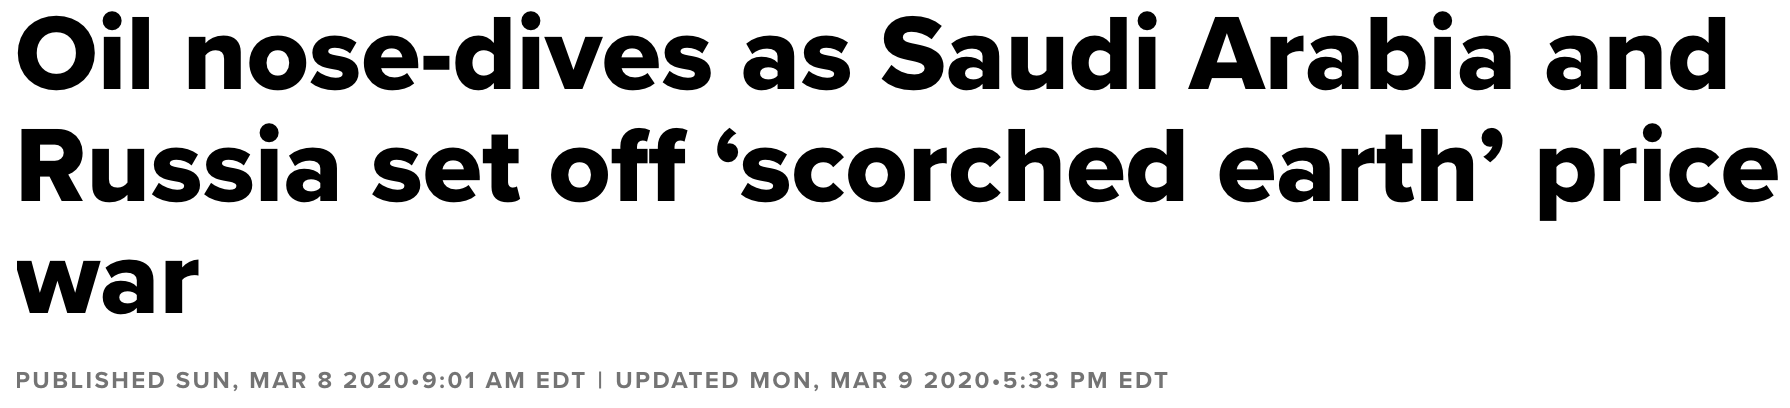
\includegraphics[scale=.3]{cnn.png}}

        \href{https://www.cnn.com/2020/03/08/investing/oil-prices-crash-opec-russia-saudi-arabia/index.html}{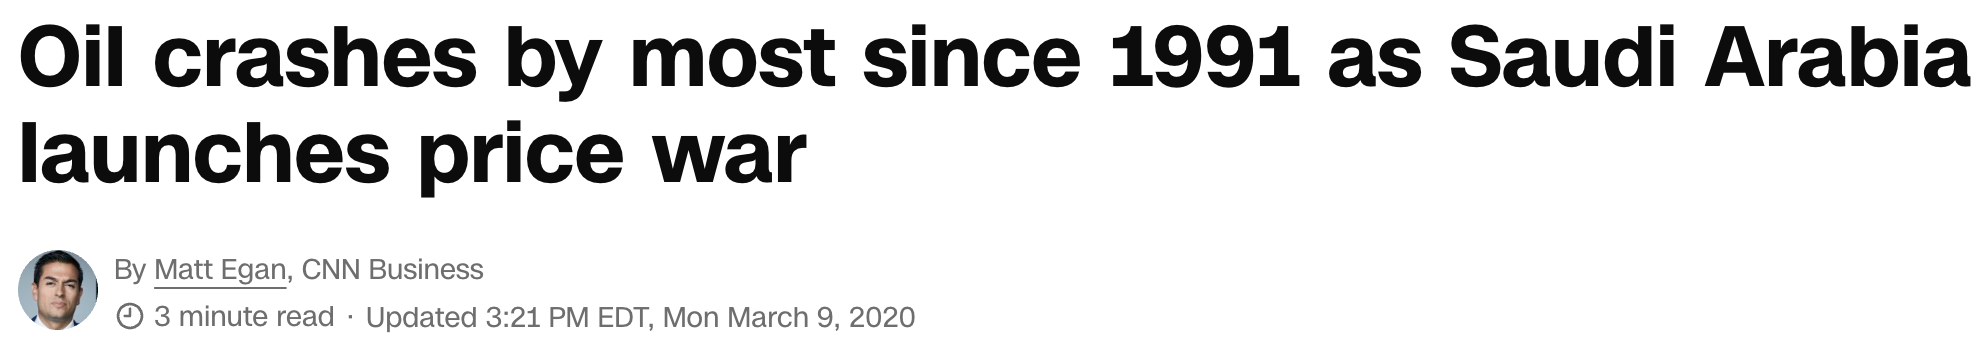
\includegraphics[scale=.3]{cnbc.png}}
        \end{example}

\end{frame}

\begin{frame}
    \frametitle{Punchline}
    
    \begin{itemize}
        \item <1-> Credible forecasting is possible under news shocks, so long as we incorporate external information to account for the \textcolor{red}{nonzero errors}. 
    \end{itemize}



    \end{frame}

\part{two}

\section{The Idea and Methodology}

\begin{frame}{Outline} % https://tex.stackexchange.com/questions/73196/beamer-table-of-contents-shade-all-previous-sections
    \tableofcontents[part=1,currentsection]\tableofcontents
\end{frame}

\begin{frame}
    \frametitle{Premise: There is breaking news at some fractional lag t-$\epsilon$}
    
    \begin{itemize}
    \item Market (i.e. crowd-sourced) mechanisms for evaluating the news are either offline, too thin, or otherwise unavailable.  They could also be simply unreliable.
    \item The \textcolor{red}{qualitative aspects} of the news provide a basis upon which to 
    \begin{itemize}
        \item match to past news shocks
        \item match in a $p$-dimensional covariate space
    \end{itemize}
    \end{itemize}
    \end{frame}


    
    % \begin{frame}
    %     \frametitle{A Primer on GARCH}
       
    %     \begin{Definition}
    
    %     Let $\{a_{t}\}$ denote an observable, real-valued discrete-time stochastic process.\\
        
    %     \bigbreak
        
    %     We call $\{a_{t}\}$ a strong GARCH process \parencite[][]{francq2019garch} with respect to $\{\epsilon_{t}\}$ iff 
    %     \begin{align*}
    %         &\sigma_{t}^{2} = \omega + \sum^{m}_{k=1}\alpha_{k}a^{2}_{t-k} + \sum_{j=1}^{s}\beta_{j}\sigma_{t-j}^{2}\\
    %         &a_{t} = \sigma_{t}\epsilon_{t}\\
    %         &\epsilon_{t} \simiid E[\epsilon_{t}]=0, Var[\epsilon_{t}] = 1\\
    %         &\forall k,j, \alpha_{k},\beta_{j}\geq 0\\ 
    %         &\forall t, \omega, \sigma_{t} > 0 
    %         \end{align*}
    
    %     \end{Definition}
    
    % \end{frame}
    
    % \begin{frame}
    %     \frametitle{Volatility Equation with an exogenous term: GARCH-X}
        
    %     \begin{align*}
    %         &\sigma_{t}^{2} = \omega+ \sum^{m}_{k=1}\alpha_{k}a^{2}_{t-k} + \sum_{j=1}^{s}\beta_{j}\sigma_{t-j}^{2} + \gamma^{T}\x_{t} \text{ .}\label{GARCH-X}
    %     \end{align*}
    
    %     We will be looking at only one exogenous term.
    
    %     \end{frame}
        
    % \begin{frame}
    %     \frametitle{Model Preliminaries}
    
    %     \fontsize{8}{7.2}
    
    %     Let $I(\cdot)$ be an indicator function.  \\
    % \bigbreak
    %     Let $T_i$ denote the time length of the time series $i$ for $i = 1, \ldots, n+1$.\\
    %     \bigbreak
    %     Let $T_i^*$ denote the largest time index prior to news shock, with $T_i^* < T_i$ (i.e. we assume at least one post-shock observation). \\
    %     \bigbreak
    %     Let $\lambda_{i,t},  \x_{i,t} \in \mathbb{R}^{d}$.  
    % \end{frame}

    \begin{frame}\frametitle{Model Setup}
    
    \fontsize{8}{7.2}
    
    For $t= 1, \ldots, T_i$ and $i = 1, \ldots, n+1$, the model $\mc{M}_1$ is defined as 

    \begin{align}
        \mc{M}_1 \colon 
    \begin{array}{l}
          y_{i,t} = F(\mathcal{F}_{i,t-1}) + \alpha_{i,t} + \epsilon_{i,t}\\[.2cm]
          \alpha_{i,t} = \x^{T}_{i,t}\lambda_{i,t} \\[.2cm]
         \x_{i,t}^{T} = (1,x^{1}_{i,t},...,x^{p}_{i,t}) \text{ (observable and deterministic w.r.t to } \mathcal{F}_{i,t-1})\\[.2cm] 
         \lambda_{i,t}^{T} = (u_{i,t},\lambda^{1}_{t},...,\lambda^{p}_{t}) \text{ (unobservable and potentially random)},\\[.2cm]
        \end{array}
    \end{align}

    \begin{align*}
    \lambda_{i,t} &\sim \mc{F}_{\lambda}\text{ with }  \E_{\mathcal{F}_{\lambda}}(\lambda) = \mu_{\lambda_{t}}, \mrm{Var}_{\mc{F}_{\lambda}}(\lambda) = \Sigma_{\lambda_{t}},\\
    \end{align*}

    and time-invariant error structure

    \begin{align*}
        \epsilon_{i,t} &\simiid \mc{F}_{\epsilon} \text{ with}  \; \E_{\mc{F}_{\epsilon}}(\epsilon) = 0, \mrm{Var}_{\mc{F}_{\epsilon}}(\epsilon)  = \sigma^{2}_{\epsilon},  \\
    \end{align*}
    
    \end{frame}

    \begin{frame}\frametitle{Model Details}
        Note that $\lambda_{i,t}^{T} = (u_{i,t},\lambda^{1}_{t},...,\lambda^{p}_{t})$
        \begin{itemize}
            
            % \item $\epsilon_{i,t}$ uncorrelated across time and donors
            \item includes the term $u_{i,t}$ that is \textcolor{blue}{not shared} among donors.
            \item is time-varying allows us to capture that most time points are without news shocks (in which case $\alpha_{i,t}$ is of negligible effect), but conditional upon information arriving between $T_{1}^{*}$ and $T_{1}^{*}+1$, we may know with near certainty that $\lambda_{1,T_{1}^{*}+h}$ will be nonzero in norm for some $h>0$. 
        \end{itemize}
    \end{frame}
    
    % \begin{frame}
    %     \frametitle{Model Details}
    %     Let $\mc{M}_{0}$ denote the subclass of $\mc{M}_{1}$ models such that $\delta \equiv 0$.  \\
    %     \bigbreak
    %     $\mc{M}_{0}$ assumes $\omega^{*}_{i,t}$ have no dependence on the covariates and are i.i.d. with $\E[ \omega^{*}_i]=\mu_{\omega^{*}}$.  
    % \end{frame}
    
    % \begin{frame}
    % \frametitle{Our Model is Nested inside a Factor Model}
    
    % \fontsize{6}{7.2}
    
    % Consider $\mc{M}_{1}$ in the context of the factor model from \cite[][]{abadie2010synthetic}, where an untreated unit is governed by:
    
    % $$Y^{N}_{i,t} = \delta_{t} + \boldsymbol\theta_{t}^{'}\textbf{Z}_{i}+\boldsymbol\lambda_{t}^{'}\boldsymbol\mu_{i}+\varepsilon_{i,t}$$
    
    % which nests the GARCH model's volatilty equation as well as the ARMA representation of a GARCH model, where
    
    % \begin{align*}
    % \delta_{t} & \sim \omega, \text{a location parameter shared across donors}\\
    % \boldsymbol\theta_{t} & \sim \boldsymbol\alpha_{k}, \text{a vector of ARCH parameters and other coefficients shared across donors} \\
    % \textbf{Z}_{i} & \sim \boldsymbol a_{i,t-k}, \text{a vector of observable quantities specific to each donor} \\
    % \boldsymbol \lambda_{t} & \sim \boldsymbol\beta_{j}, \text{a vector of GARCH parameters shared across donors} \\
    % \boldsymbol \mu_{i} & \sim \boldsymbol \sigma_{i,t-j}^{2}, \text{a vector of latent quantities specific to each donor}   \\
    % \end{align*}
    
    % % and $\varepsilon_{i,t}$ is idiosyncratic noise, uncorrelated across time and donors.
    % \end{frame}
     
    \begin{frame}
        \frametitle{Significance of the Covariates $\x_{i,t}$}
        Covariates chosen for inclusion may be any $\mathcal{F}_{t}$-measurable function, for example
        \begin{itemize}
            \item levels
            \item differences in levels
            \item log returns
            \item percentage returns
            \item measurable transformations of the above
        \end{itemize}
    
        \bigbreak 
    
        Key criterion for inclusion: how plausible is the covariate as a \textcolor{red}{proxy for risk conditions} for the time series under study?
    \end{frame}
    
    % \begin{frame}
    % \frametitle{Realized Volatility Estimation}
    
    % Examine $K$ units of of time; each unit is divided into $m$ intervals of length $\frac{1}{m}$.  Let $p_{t} = \log{P_{t}}$, and let $\tilde{r}(t,\frac{1}{m}) = p_{t} - p_{t-\frac{1}{m}}$  \parencite[][]{andersen2008realized}. 
    
    % \bigbreak
    
    % Estimate variance of $i$th log return series using Realized Volatility of the $K$ consecutive trading days that conclude with day $t$, denoted $RV_{i,t}^{K,m}$, using
    
    % $$RV_{i,t}^{K,m} = \frac{1}{K}\sum^{Km}_{v=1}\tilde{r}^{2}(v/m,1/m),$$
    
    % where the $K$ trading days have been chopped into $Km$ equally-sized blocks.
    
    % Assuming the $K$ units $\tilde{r}(t, 1) = p_{t} - p_{t-1}$ are s.t. $\tilde{r}(t, 1) \simiid N(\mu, \delta^{2})$, it is easily verified that 
    
    % $$\E[RV^{K,m}] = \frac{\mu^{2}}{m} + \delta^{2},$$
    % which is a biased but consistent estimator of the variance.  We pick $m = 77$, corresponding to the 6.5-hour trading day chopped into 5-minute blocks, omitting first five-minutes of the day.
    
    % \end{frame}
    
    
    \begin{frame}
    \frametitle{Forecasting}
    
    \fontsize{7.6}{7}
        
    We now present two one-step-ahead forecasts.  First is the unadjusted forecast. The second is the adjusted forecast, which differs by the predicted correction term:

    \begin{align*}
      \text{Forecast 1: } 
       &\hat y_{unadjusted, T_{1}^{*}+1} = \hat\E[y_{1,T_{1}^{*}+1}|\mathcal{F}_{T_{1}^{*}}] \\
       \\
      \text{Forecast 2: }
       &\hat y_{adjusted,T_{1}^{*}+1} = \hat\E[y_{1,T_{1}^{*}+1}|\mathcal{F}_{T_{1}^{*}}] + \hat\alpha_{T^{*}_{1}+1} \text{ .}
    \end{align*}

    \end{frame}
    
    \begin{frame}
    \frametitle{Distance-based Weighting in Action}

    (For ease of exposition, we omit time indices)\\
    
        \bigskip

    \begin{itemize}
    
    \item <1->  Observe the pair $(\{\hat\alpha_{i}\}^{n+1}_{i=2},\{\x_{i}\}^{n+1}_{i=2})$.  \\
    
    \item <2-> Goal: recover weights $\{\weight_{i}\}^{n+1}_{i=2} \in \Delta^{n}$ and compute $\hat\alpha \coloneq \sum^{n+1}_{i=2}\weight_{i}\hat\alpha_{i}$, our predicted correction term (more about this later).
    
    \item <3-> Following \cite[][]{abadie2003economic},\cite[][]{abadie2010synthetic}, let $\|\cdot\|_{\textbf{S}}$ denote any semi-norm on $\mathbb{R}^{p}$, and define
    
    
    \begin{align*}
    \{\pi\}_{i=2}^{n+1} = \argmin_{\pi}\|\textbf{v}_{1,T^{*}} - \V_{T^{*}}\pi \|_{\textbf{S}} \text{ .}
    \end{align*}
    
    % Nota bene: the weights $\{\weight_{i}\}_{i=2}^{n+1}$ are deterministic with respect to $\mathcal{F}_{T^{*}}$.
    
    \end{itemize}
    \end{frame}

% \begin{frame}
%     \frametitle{My Prelim: An incredibly Brief Recap}

%     \begin{tikzpicture}[edge from parent path={[<-,line width=2pt,green!50!black](\tikzparentnode) -- (\tikzchildnode)},
%         level 1/.style = { level distance = 40mm,
%                            sibling distance = 45mm},
%         level 2/.style = { level distance = 53mm,
%                            sibling distance = 30mm}, 
%         treenode/.style = {shape = rectangle,
%           rounded corners, draw,
%           top color=white, bottom color=blue!30},
%         every child node/.style = {treenode},
%         engine/.style = {inner sep=1pt, font = \tiny, sloped, above},
%         grow = left
%       ]
%       \node [treenode] {Adjusted forecast}
%         child { node {Weighted Donor Fixed Effects}
%           child { node {Time Series Under Study} edge from parent node[engine] {Series and covariates}}
%           child { node {Donor pool} edge from parent node[engine] {Fixed effect estimates} }
%           child { node {Covariate Choices} edge from parent node[engine] {}}
%         }
       
%       ;
%       \end{tikzpicture}

% \end{frame}

\begin{frame}
\frametitle{Visuals That Tell The Story}

\begin{tikzpicture}[
    > = stealth, % arrow head style
    shorten > = 2.2pt, % don't touch arrow head to node
    auto,
    node distance = 5.8cm, % distance between nodes
    semithick % line style
]

\tikzstyle{every state}=[
    draw = black,
    thick,
    fill = white,
    minimum size = 4mm
]
\node[state, fill = yellow] (Target Series) {Target Series};
\node[state, fill = orange] (Donor Pool) [above of = Target Series] {Donor Pool};

\node[rectangle, rounded corners, draw=blue!80, line width=.2mm, inner sep=0pt,minimum size=14pt]   (Distance-based Weighting) [above right of=Target Series] {Distance-based Weighting};

\node[state] (Donors) [below right of=Target Series] {Donors};
\node[state, fill = pink] (Adjusted Forecast) [right of=Distance-based Weighting] {Adjusted Forecast};

\path[->] (Target Series) edge node {Pre-Shock Covariates} (Distance-based Weighting);
\path[->] (Target Series) edge [bend right] node {Unadjusted Forecast} (Adjusted Forecast);
\path[->] (Donor Pool) edge [bend left] node {Pre-Shock Covariates} (Distance-based Weighting);
\path[->] (Donor Pool) edge [left] [bend right] node {FE estimates} (Distance-based Weighting);
 \path[->] (Distance-based Weighting) edge [below] [bend right] node {Predicted Correction Function} (Adjusted Forecast);


%\draw[red, dashed] (1, 2) -- (1, -2);
\end{tikzpicture}

\end{frame}

\begin{frame}\frametitle{Visuals That Tell The Story}
    The forecaster's decision tree

    \begin{figure} 
        \centering  
      \resizebox{\textwidth}{!}{%
      \begin{forest}
        /tikz/every node/.append style={font=\small},
        for tree={
          rounded corners, 
          % top color=gray!5, bottom color=gray!30, 
          edge+={darkgray, line width=4pt}, 
          draw=darkgray, 
          l sep=.8cm,
          s sep=.5cm,
          minimum height=8.8cm,
          minimum width=1cm,
          child anchor=west,
          parent anchor=east,
          grow'=east,
        minimum size=1cm,%new possibility
        text width=4cm,%
          draw,
          anchor=west,
          edge path={
            \noexpand\path[\forestoption{edge}]
              (.child anchor) -| +(-5pt,0) -- +(-5pt,0) |-
              (!u.parent anchor)\forestoption{edge label};
          },
        }
          [Break in the DGP between $T^{*}$ and $T^{*}+1$?,fill=blue!30 
              [Is there information outside of “regular forces”,edge=green, fill=blue!30,draw=green
                  [Can we use the information outside “regular forces” to forecast (as opposed to merely spotting the break)?,edge=green,,fill=blue!30 
                      [Do you have a parametric model (with estimable parameters) for how information outside of ``regular forces” will figure at $T^{*}+h$?,edge=green,fill=blue!30 
                        [What other time series are governed by the parametric model? 
                        ,edge=green,fill=blue!30 
                        ]
                        [The information that helped spot the break can be used.
                        ,edge=red,fill=gray!30
                        ]
                        ]
                      [Use “regular forces” to do the model adjustment.,edge=red,fill=gray!30
                      ]
                      ]
                      [Then forecasting will require at least one post-break data point to be observed.,edge=red,fill=gray!30]
                  ]
                  [\cite{clements1998forecasting} discuss this.,edge=red,fill=gray!30]
                  ]
              ]
          ]
      \end{forest}
      }\caption{Forecast Model Adjustment: A Decision Tree}\label{fig:tree}
      \end{figure}

\end{frame}

\begin{frame}\frametitle{Visuals That Tell The Story}

%https://tex.stackexchange.com/questions/174317/creating-a-labeled-tetrahedron-with-tikzpicture
\begin{figure}
    \centering
    \begin{tikzpicture}[line join = round, line cap = round]
    \pgfmathsetmacro{\factor}{1/sqrt(2)};
    \coordinate [label=right:Donor 1] (1) at (2,0,-2*\factor);
    \coordinate [label=left:Donor 2] (2) at (-2,0,-2*\factor);
    \coordinate [label=above:Donor 3] (3) at (0,2,2*\factor);
    \coordinate [label=below:Donor 4] (4) at (0,-2,2*\factor);
    \coordinate [label=below:$\vec{\pi}_{MSE minimizer}$] (5) at (1.7,-.8,-.3*\factor);
    
    
    % \draw[->] (0,0) -- (3,0,0) node[right] {$x$};
    % \draw[->] (0,0) -- (0,3,0) node[above] {$y$};
    % \draw[->] (0,0) -- (0,0,3) node[below left] {$z$};
    \foreach \i in {1,2,3,4}
        \draw[dashed] (0,0)--(\i);
    \draw[-, fill=red!30, opacity=.3] (1)--(4)--(2)--cycle;
    \draw[-, fill=green!30, opacity=.3] (1) --(4)--(3)--cycle;
    \draw[-, fill=purple!30, opacity=.3] (2)--(4)--(3)--cycle;
    \end{tikzpicture}
    \caption{The 3-Simplex, $\Delta^{3}$, where hypothetical minimizer is a convex combination of Donors 1 and 4.}
    \end{figure}
    
\end{frame}

\begin{frame}\frametitle{Three slides about theory}
   
    \begin{table}[htb]
        \centering % instead of \begin{center}
        \caption{A 2x2 Schema of Forecast Information, With Examples}
        \begin{tabular}{ | p{1cm} | p{4.8cm}| p{4.8cm} | } 
          \hline
          & Conventional Econometric Models & Outside Conventional Econometric Models\\ 
          \hline
          internal & \textcolor{blue}{Lags of the series itself; past shocks}  & Polynomial expansion of the feature space and other transformations without solid theoretical motivation \\
          \hline
          external & Macro variables like interest rates, commodity prices; weather-related variables & Google Trends, high-frequency data like prediction markets; past shocks under similar conditions \\ 
          \hline
        \end{tabular}
      \end{table}
\end{frame}

\begin{frame}\frametitle{Three slides about theory}
   
    \begin{table}[htb]
        \centering % instead of \begin{center}
        \caption{A 2x2 Schema of Forecast Information, With Examples}
        \begin{tabular}{ | p{1cm} | p{4.8cm}| p{4.8cm} | } 
          \hline
          & Conventional Econometric Models & Outside Conventional Econometric Models\\ 
          \hline
          internal & Lags of the series itself; past shocks & \textcolor{blue}{Polynomial expansion of the feature space and other transformations without solid theoretical motivation} \\
          \hline
          external & Macro variables like interest rates, commodity prices; weather-related variables & Google Trends, high-frequency data like prediction markets; past shocks under similar conditions \\ 
          \hline
        \end{tabular}
      \end{table}
\end{frame}
\begin{frame}\frametitle{Three slides about theory}
   
    \begin{table}[htb]
        \centering % instead of \begin{center}
        \caption{A 2x2 Schema of Forecast Information, With Examples}
        \begin{tabular}{ | p{1cm} | p{4.8cm}| p{4.8cm} | } 
          \hline
          & Conventional Econometric Models & Outside Conventional Econometric Models\\ 
          \hline
          internal &  Lags of the series itself; past shocks & Polynomial expansion of the feature space and other transformations without solid theoretical motivation \\
          \hline
          external & \textcolor{blue}{Macro variables like interest rates, commodity prices; weather-related variables} & Google Trends, high-frequency data like prediction markets; past shocks under similar conditions \\ 
          \hline
        \end{tabular}
      \end{table}
\end{frame}
\begin{frame}\frametitle{Three slides about theory}
   
    \begin{table}[htb]
        \centering % instead of \begin{center}
        \caption{A 2x2 Schema of Forecast Information, With Examples}
        \begin{tabular}{ | p{1cm} | p{4.8cm}| p{4.8cm} | } 
          \hline
          & Conventional Econometric Models & Outside Conventional Econometric Models\\ 
          \hline
          internal & Lags of the series itself; past shocks & Polynomial expansion of the feature space and other transformations without solid theoretical motivation \\
          \hline
          external & Macro variables like interest rates, commodity prices; weather-related variables & \textcolor{blue}{Google Trends, high-frequency data like prediction markets; past shocks under similar conditions} \\ 
          \hline
        \end{tabular}
      \end{table}
\end{frame}

\begin{frame}\frametitle{Three slides about theory}
   
    An oft-abused term in applied math: similarity
    \begin{itemize}
    \item Quantitative or qualitative?
    \item Approximation-based?
    \item Symmetric or asymmetric?
    \item Binary or $n$-ary?
    \end{itemize}

\end{frame}

\begin{frame}\frametitle{Three slides about theory}
   
    An oft-abused term in applied math: similarity
    \begin{itemize}
    \item Quantitative or qualitative?
    \item Approximation-based?
    \item Symmetric or asymmetric?
    \item Binary or $n$-ary?
    \end{itemize}

    To give a name to what we're doing, we can call it \textcolor{blue}{distance-based weighting}, which is a special case of an approximation-based $n$-ary similarity metric.
\end{frame}

\begin{frame}\frametitle{Three slides about theory}
    The term $\x^{T}_{i,t}\lambda_{i,t}$ is deemed the $\textcolor{blue}{correction} \text{ } \textcolor{blue}{term}$ for donor $i$ at time $t$, and the function

    \begin{align*}
      \xi \colon \mathcal{F}_{2,T^{*}_{2}+h} \times \ldots \times \mathcal{F}_{n+1, T^{*}_{n+1}+h} &\to \mathcal{F}_{1,T^{*}_{1}+h}\\
    \end{align*}
    that estimates or predicts $\alpha_{1,T^{*}_{1}+h}$ will be deemed the \textcolor{red}{correction function}.  
    
    \bigskip 
    
    The correction function maps donor information --- be it observables or inferences --- to the prediction function for the time series under study. 
\end{frame}

\begin{frame}\frametitle{Global Overview}

    Abstracting away from particular models, what does our method require?

    \begin{enumerate}
        \item <1-> \textbf{Object-to-predict}
       Random object (indexed over time and possibly space, as well) obeying specification with additive errors 
            
      \item <2-> \textbf{Common Model Family on the Shocks} Requires that residuals be governed by a model that is shared across all units.  
      
      \item<3->  \textbf{Reliable and Shared Model-Fitting Procedure} There must exist a reliable model-fitting procedure for the $n+1$ units.
      
      \item<4-> \textbf{Reliable Correction Term Estimation} 

      \item<5->  \textbf{Reliable Correction Function Estimation} There must exist a correction function (presumably based on the correction term) that maps data from the donor pool to the $\textit{predicted}$ correction term in the time series under study based on similarity.  
    \end{enumerate}
\end{frame}

\section{Formal Results}

\begin{frame}\frametitle{Do we have theoretical guarantees?}

    We do!

    \bigskip

    Our formal results fall into the following buckets:

    \begin{enumerate}
        \item convergence in distribution results
        \item consistency results
        \item asymptotic loss
    \end{enumerate}

Here we share only the first two, and for both GARCH and AR($p$) models.

    \end{frame}

\begin{frame}\frametitle{GARCH - Formal Results}
        
     
\begin{prop}\label{omega_consistency}
    Assume
    \begin{enumerate}
      \item For each $i$, $1\leq i \leq n$, $\{a_{i,t}\}_{t=0,...,T_i}$ obeys a GARCH-X($m,s$), with volatility shocks found in $\mc{M}_{1}$, where $T_i$ is the length of the $i$th series.
      \item For each $i, \{\omega_{i,t}^{*}\}_{t=0,...,T_i}$ is potentially non-zero at $\{T^{*}_{i}+1,... ,T^{*}_{i}+L_{i}^{vol}\}$, $\omega_{i,T_{i}^{*}+1}^{*}\equiv...\equiv\omega_{i,T_{i}^{*}+L_{i}^{vol}}^{*}$, and zero otherwise, where the arrival of $T_{i}^{*}$ is governed by a time-invariant distribution on $\{a_{i,t}\}_{t=0,...,T_i-1}$, and both the arrival and conclusion of the shock is observable by the researcher. \label{stationarity_of_omega_i_t}
      \item The conditions in Assumption 0 of \cite[][]{han2014asymptotic} hold.
    \end{enumerate}

    Then for any $i, 1\leq i \leq n+1$, and for any $r, 1\leq r \leq L_{i}^{vol}$, $\hat\omega_{i,T_{i}^{*}+r}^{*} \overset{p}{\longrightarrow} \omega_{i,T_{i}^{*}+r}^{*}$ as $t\rightarrow\infty$.  Additionally, $\hat\omega_{i,*}^{*} \overset{d}{\longrightarrow} \omega_{i,T_{i}^{*}+r}^{*}$ as $t\rightarrow\infty$, and if for all $i, 1 \leq i \leq n+ 1$, $u_{i,t} \equiv 0$ on $\{T^{*}_{i}+1,... ,T^{*}_{i}+L_{i}^{vol}\}$, then $\hat\omega_{i,T_{i}^{*}+r}^{*} \overset{p}{\longrightarrow} \omega_{i,T_{i}^{*}+r}^{*}$ .
    \end{prop}

    In plain language, this result gives us distributional results about our correction terms as we estimate over arbitrarily long horizons.

\end{frame}
    
    \begin{frame}\frametitle{GARCH - Formal Results} 
    Having established the consistency of the estimators $\hat\omega^{*}_{i,T_{i}^{*}+r}$, we extend that result to prove asymptotic properties of the conditional forecast function itself.
    
      \begin{prop}\label{sigma_consistency}
        Assume
        \begin{enumerate}
          \item All conditions listed in the preceding proposition \ref{omega_consistency}.
          \item There exist weights $\{\pi_{i}\}_{i=2}^{n+1}$ such that $\textbf{v}_{1,T_{1}^{*}} = \sum^{n+1}_{i=2}\weight_{i} \textbf{v}_{i,T_{i}^{*}}$.
         \end{enumerate}
      Then for any $r$, $1\leq r \leq L_{1}^{vol}$, $\hat\sigma^{2}_{adjusted,T_{1}^{*}+r}\overset{d}{\longrightarrow}\sigma^{2}_{1,T_{1}^{*}+r}$ as $t\rightarrow\infty$ in the donor pool, and if for all $i, 1 \leq i \leq n+ 1$, $u_{i,t} \equiv 0$ on $\{T^{*}_{i}+1,... ,T^{*}_{i}+L_{i}^{vol}\}$, then $\hat\sigma^{2}_{adjusted,T_{1}^{*}+r}\overset{p}{\longrightarrow}\sigma^{2}_{1,T_{1}^{*}+r}$.
      \end{prop}

      In plain language, our volatility prediction have a known distribution, by virtue of our correction terms have a known distribution.

\end{frame}

\section{Applications}

\begin{frame}
    \frametitle{An inventory of models}

    \begin{itemize}
        \item <1-> GARCH (paper is under review at the \textit{International Journal of Forecasting})
        \item <2-> HAR (to be submitted in the coming weeks as part of second paper)
        \item <3-> Exponential Shocks (to be submitted in the coming weeks as part of second paper)

    \end{itemize}
\end{frame}

\begin{frame}
    \frametitle{GARCH Volatility Forecasts}
    The least you need to know here: GARCH is the premier volatility modeling family for daily data.

    \bigskip

    We demonstrate our method's usefulness with an easy-to-approach example.
\end{frame}

% \begin{frame}
%     \frametitle{My Prelim: An Incredibly Brief Recap}

%     \begin{itemize}
%         \item <1-> Paper is under review at the \textit{International Journal of Forecasting}
%         \item <2-> Event-driven investing strategies (unscheduled news shock)
%         \item <3-> Scheduled macroeconomic news possibly pre-empted by a news leak

%         \href{https://www.wsj.com/articles/bad-inflation-reports-raise-odds-of-surprise-0-75-percentage-point-rate-rise-this-week-11655147927}{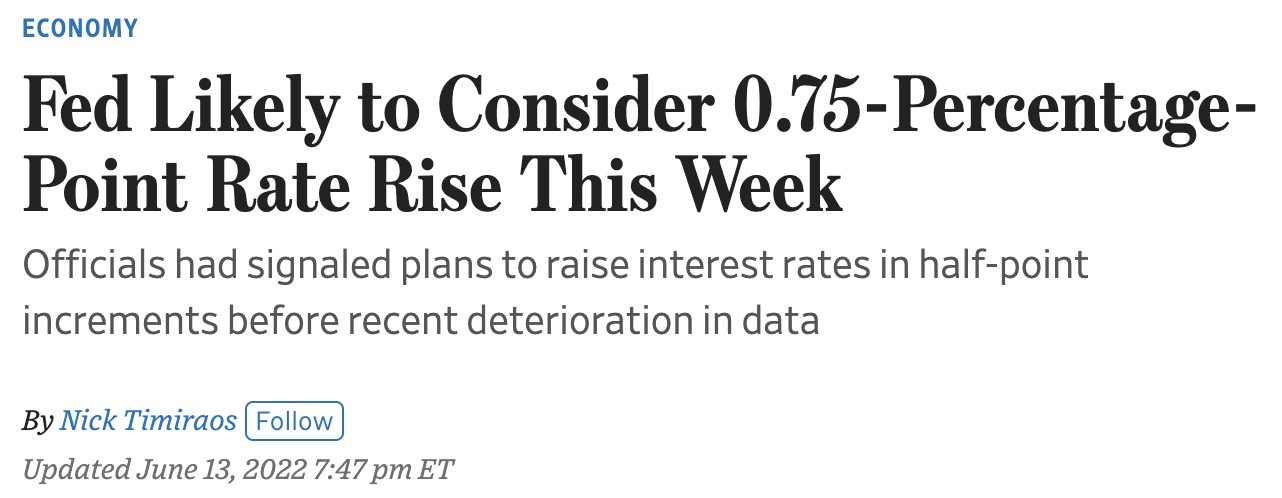
\includegraphics[scale=.3]{WSJ_rate_hike_2022.png}}

%     \end{itemize}
% \end{frame}
    
    \begin{frame}{Why apply our method to the 2016 US Election?}
    
        \begin{itemize}
            \item You can win the US Presidency without a majority.
            \item No incumbent candidate
            \item Donald J. Trump espoused unorthodox, populist positions on healthcare, trade, foreign policy
            \item Donald J. Trump had no record to assess or criticize
            \item It was not predicted -- hence it delivered news.
        \end{itemize}
        
    \end{frame}
    \begin{frame}
        \begin{figure}[H]
            \begin{center}
              
\includegraphics[scale=.2]{iyg.png}
              \caption{IYG includes JPM, BAC, WF, CITI, among other financial majors}
              \end{center}
            \end{figure}
    \begin{enumerate}
        \item \textbf{Model choice} GARCH(1,1) on the daily log return series of IYG in each donor
    
        \item \textbf{Covariate Choice} 
        \begin{itemize}
            \item previous 30 log returns of IYG (large pre-treatment period, in the language of SC)
            \item log return Crude Oil (CL.F)
            \item VIX
            \item log return of the VIX
            \item log returns of the 3-month, 5-year, 10-year, and 30-year US Treasuries
            \item return of the most recently available monthly spread between AAA and BAA corporate debt
            \item log return in the trading volume of the ETF IYG itself
        \end{itemize}
    
        \item \textbf{Donor pool construction} US Elections from 2004, 2008, 2012
    
        \item \textbf{Choice of estimator for volatility} Sum of 77 squared five-minute returns generated between 9:35am and 4pm on November 9th, 2016.
    \end{enumerate} 
    
    \end{frame}
    
    \begin{frame}{2016 Election}
        \begin{figure}[H]
            \begin{center}
              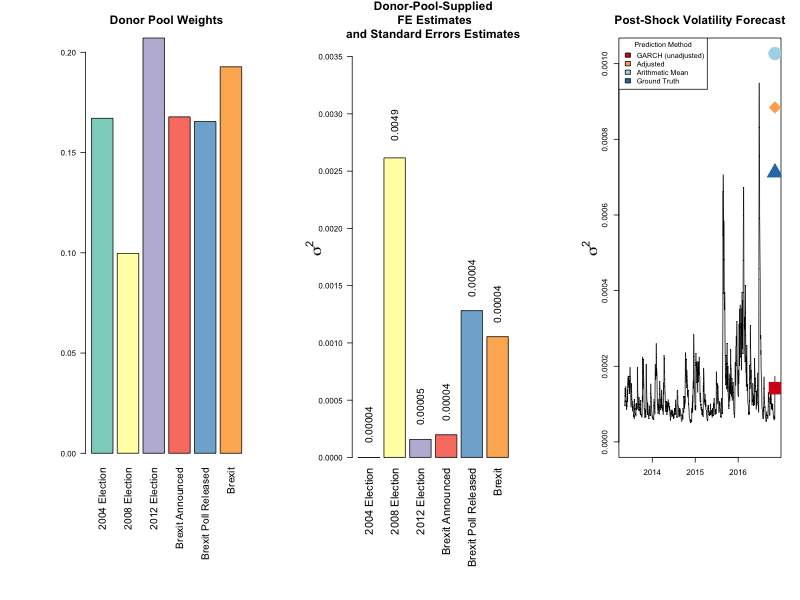
\includegraphics[scale=.34]{real_data_output_plots/TueSep241059512024_IYG_None_None.png}
              \caption{The volatility induced by the 2016 US election}
              \label{fig:SVF_2016}
              \end{center}
            \end{figure}
    \end{frame}

% \begin{frame}
%     \frametitle{The Post-prelim Direction of my research}
    
%     \begin{itemize}
%         \item Extending similarity-based parameter correction to the state-of-the-art HAR model 
%         \item Extending similarity-based parameter correction to non-linear shock models
%         \item Building out a general framework for parameter correction 
%     \end{itemize}
% \end{frame}



% \begin{frame}
%     \frametitle{Background and related methods}
%     Volatility Modeling

%     \begin{itemize}
%         \item GARCH is slow to react to shocks \parencite[][]{andersen2003modeling}
%         \item Asymmetric GARCH models catch up faster but need post-shock data
%         \item Realized GARCH \parencite[][]{hansen2012realized}, in our setting, would require post-shock information and/or high-frequency data in order to outperform, and Realized GARCH is highly parameterized
%     \end{itemize}
% \end{frame}

% \begin{frame}
%     \frametitle{Background and related methods}

%     Forecast Adjustment
%     \begin{itemize}
%         \item \cite[][]{clements1996intercept,clements1998forecasting} laid the groundwork for modeling nonzero errors in time series forecasting
%         \item \cite[][]{guerron2017macroeconomic} use a series' own errors to correct the forecast for that series
%         \item \cite[][]{dendramis2020similarity} use a similarity-based procedure to correct $\hat\beta$ in time series forecasts
%         \item \cite[][]{foroni2022forecasting} adjust pandemic-era forecasts using intercept correction techniques and data from Great Financial Crisis
%         \item \cite[][]{lin2021minimizing} use distanced-based weighting (a similarity approach) to aggregate and weight fixed effects from a donor pool
%     \end{itemize}
% \end{frame}

% \begin{frame}{What we will discuss in this section}
%     \begin{enumerate}
%     \item Role of outside information
%     \item The Meaning and Use of Similarity 
%     \end{enumerate}
% \end{frame}

% \begin{frame}{Hypotheses to Test Via Simulations}
%     Ceteris paribus...
%     \begin{enumerate}
%         \item <1-> Distance-based weighting should \textcolor{red}{outperform} the unadjusted forecast as $\textcolor{blue}{\delta}$ increases (signal-to-noise)
%         \item <2-> Distance-based weighting should \textcolor{red}{underperform} as the variability in $\textcolor{blue}{u_{i,t}}$ increases (signal-to-noise)
%         \item <3-> Distance-based weighting should \textcolor{red}{outperform} the arithmetic mean as the variability of $\textcolor{blue}{\textbf{v}_{i,T^{*}}}$ increases between donors (importance of linear signal)
%         \item <4-> Distance-based weighting should \textcolor{red}{underperform} the arithmetic mean as $\textcolor{blue}{\mu_{\omega^{*}}}$ increases (importance of linear signal)
%         \item <5-> When $D^{return}_{i,T^{*}+1} = 1 = D^{vol}_{i,T^{*}+1}$, i.e. when there is both a \textcolor{red}{return shock} and \textcolor{red}{volatility shock}, our adjustment methods should \textcolor{red}{underperform} due to failed identification in $a_{T^{*}+1} = \sigma_{T^{*}+1}\epsilon_{T^{*}+1}$
%     \end{enumerate}
% \end{frame}



% \begin{frame}
%     \fontsize{8pt}{9pt}
    
%     \begin{figure}[h!]
%       \begin{center}
%         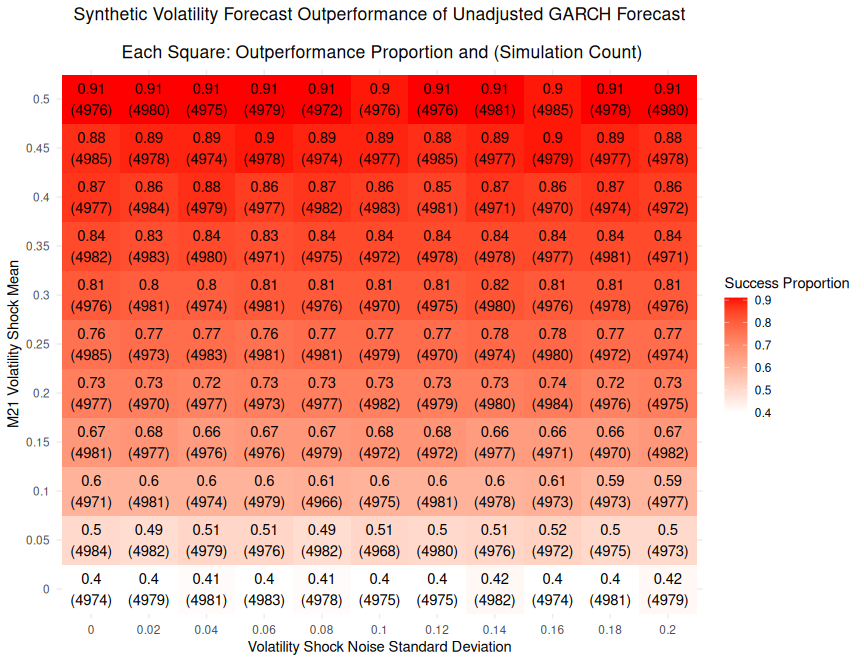
\includegraphics[scale=.29]{simulation_plots/standard_simulation_alpha_.1_beta_.82.png}
%         \caption{Fixed parameter values: $\alpha = .1, \beta = .82, \mu_{x} = 1, \sigma_{x} = .1$}\label{fig:heavy_beta}
%       \end{center}
%       \end{figure}

% \end{frame}

% \begin{frame}
%     \fontsize{8pt}{9pt}

%     If we switch the values of $\alpha$ and $\beta$, we see similar behavior. 
%     \begin{figure}[h!]
%       \begin{center}
%         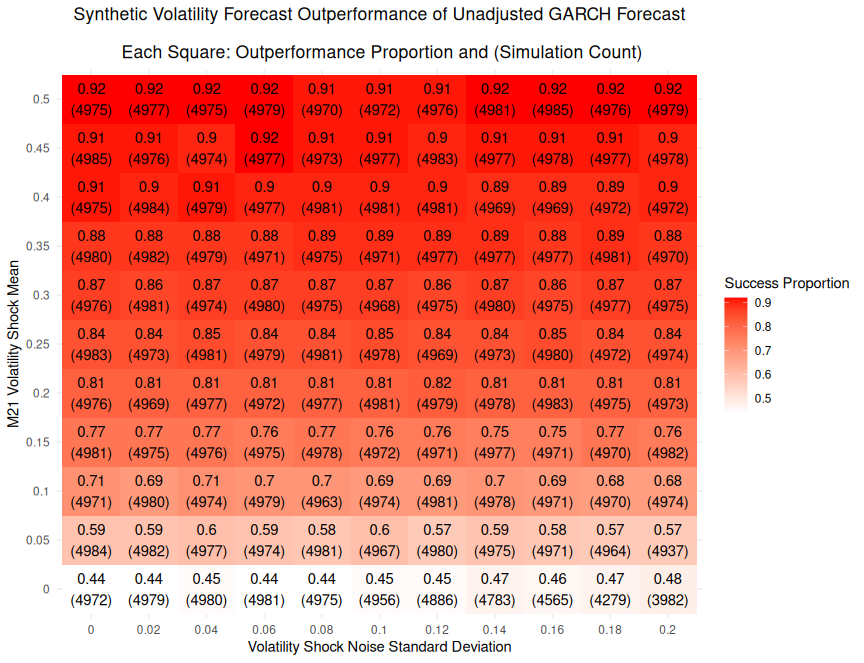
\includegraphics[scale=.29]{simulation_plots/standard_simulation_alpha_.82_beta_.1.png}
%         \caption{Fixed parameter values: $\alpha = .82, \beta = .1, \mu_{x} = 1, \sigma_{x} = .1$}
%         \label{fig:heavy_alpha}
%       \end{center}
%       \end{figure}

% \end{frame}

\begin{frame}
    \fontsize{8pt}{9pt}
    
    \frametitle{Heterogeneous Autoregression (HAR)}
    
    \begin{figure}[h!]
        \centering    
        \movie[externalviewer]{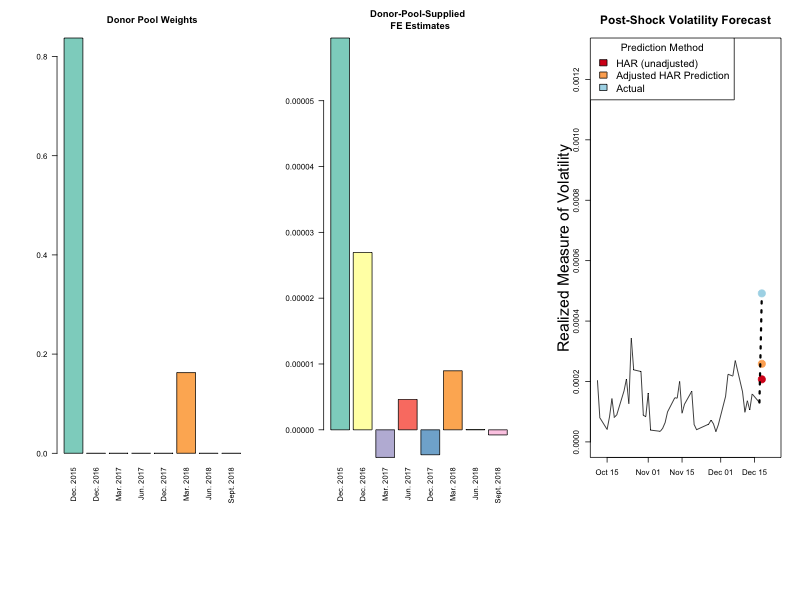
\includegraphics[scale=.3]{real_data_output_plots/savetime_SatJun151644072024__^VIX-^IRX-^XAU_^VIX_2018-12-18-2015-12-15-2016-12-13-2017-03-14-2017-06-13-2017-12-12-2018-03-20-2018-06-12-2018-09-25.png}}{demonstration.mp4}
            \caption{Click the image above to see a video of the R package's functionality.}
        \end{figure}     

    \end{frame}


\begin{frame}
    \fontsize{8pt}{9pt}
    
    \frametitle{Simulations: Parameter Correction Using An Aggregated Decay Parameter from Donors}
    
        
    Recall an \hyperlink{model_1}{$\mc{M}_1$} model on the volatility, which is characterized by an exogenous shock to the volatility equation generated by an affine function of the covariates.

    \bigskip

    Now consider, for $i=1,2,...,n+1$, the family of models
    
    \begin{align}
        \mc{M}_{exp} \colon 
    \begin{array}{l}
        y_{i,t} = \alpha_{i} + \eta[1 - e^{-\psi_{i}[t-T_{i}^{*}]}]\textbf{1}_{t\geq T_{i}^{*}+1} + \epsilon_{i,t}, \epsilon_{i,t} \\[.2cm]  
          \psi_{i} = \x^{T}_{i,t}\lambda_{i,t} \\[.2cm]
         \x_{i,t}^{T} = (1,x^{1}_{i,t},...,x^{p}_{i,t})\\[.2cm] 
         \lambda_{i,t}^{T} = (u_{i,t},\lambda^{1}_{t},...,\lambda^{p}_{t}),\\[.2cm]
        \end{array}
    \end{align}

    with time-varying and observable covariate vector $\x_{i,t}^{T}$, time-varying, unobservable, and potentially random vector
    
    \begin{align*}
    \lambda_{i,t} &\sim \mc{F}_{\lambda}\text{ with }  \E_{\mathcal{F}_{\lambda}}(\lambda) = \mu_{\lambda_{t}}, \mrm{Var}_{\mc{F}_{\lambda}}(\lambda) = \Sigma_{\lambda_{t}},\\
    \end{align*}

    and time-invariant error structure just as in $\mc{M}_{1}$.

    % https://www.overleaf.com/learn/latex/Beamer_Presentations%3A_A_Tutorial_for_Beginners_(Part_3)%E2%80%94Blocks%2C_Code%2C_Hyperlinks_and_Buttons

    \end{frame}

    \begin{frame}
        \fontsize{8pt}{9pt}
        
        \frametitle{Simulations: Parameter Correction Using An Aggregated Decay Parameter from Donors}
    \begin{figure}[h!]
      \begin{center}
        \begin{tikzpicture}
          \node[anchor=south west,inner sep=0] at (0,0) {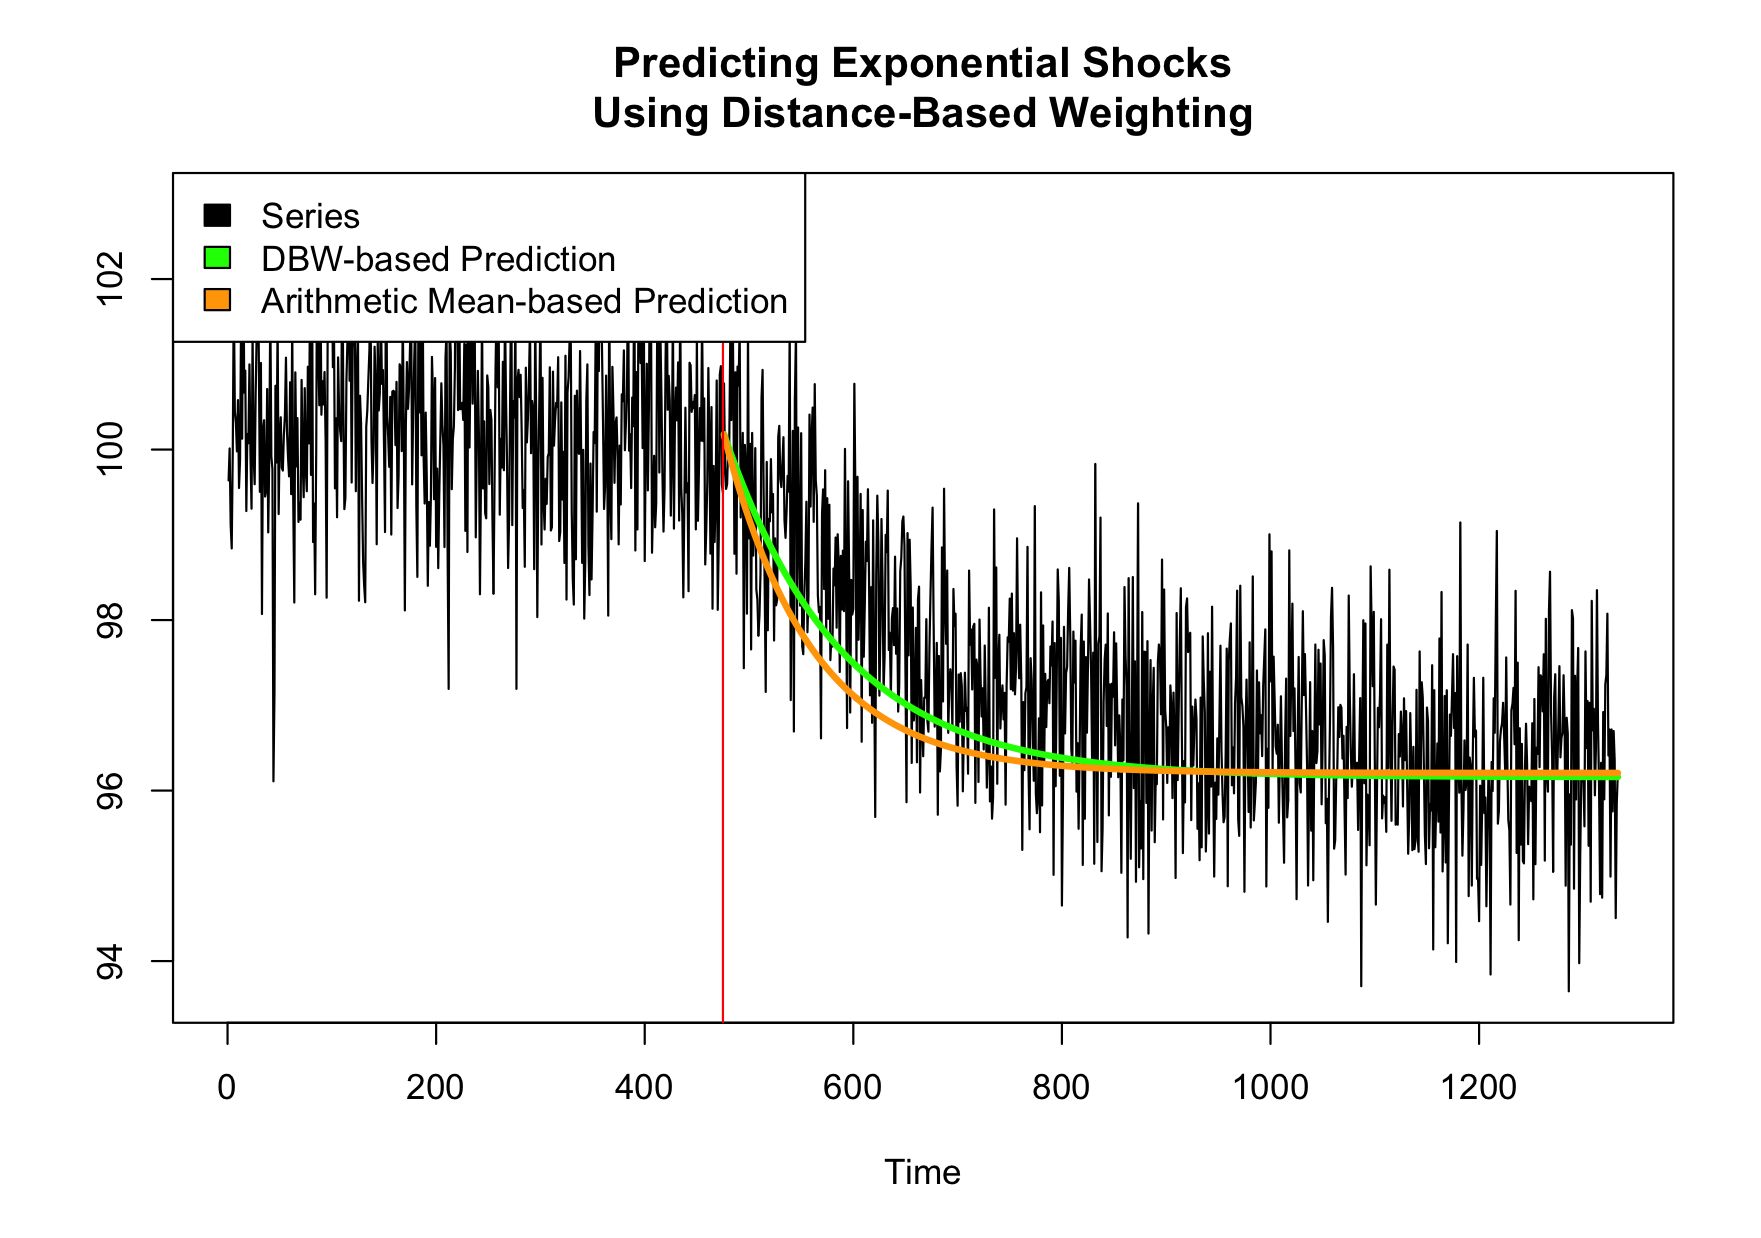
\includegraphics[scale = .11]{exponential_sim_plot.png
          }};
          % \draw[red,ultra thick,rounded corners] (7.5,5.3) rectangle (9.4,6.2);
          % \node[draw,text width=4.45cm] at (9.8,3.2) {$\textcolor{blue}{\hat\sigma^{2}_{adjusted} = \hat\sigma^{2}_{unadjusted} + \hat\omega^{*}}$ };
          % \node[draw,text width=2.62cm] at (14.8,2.8) {$\textcolor{blue}{\hat\omega^{*} = \sum^{n+1}_{i=2}\pi_{i}\hat\omega^{*}_{i}}$ };    
          
      \end{tikzpicture}
        \caption{Simulated random walk centered at $\mu = 100$, subject to a shock at approximately time index 440.  Shock of size -4 is not realized over a single index.  Instead, shock is governed by a decay exponential decay parameter $\psi_{1}$, as are exponential shocks in $n = 10$ donor series.  We estimate $\psi_{1}$ using a convex combination of the estimated decay parameters $\{\psi_{i}\}_{i=2}^{n+1}$ , resulting in a distance-based weighting prediction of the shock.  We also illustrate the arithmetic-mean-based prediction of the shock using the color orange.  This prediction is based on an overestimate of $\psi_{1}$ and hence results in residuals that undershoot the time series under study.} 
     
        \end{center}
      \end{figure}
      
    \end{frame}

\section{Software and LLMs}

\begin{frame}\frametitle{Software}
    R package

    % \movie[showcontrols]{rec2.mp4}

    \begin{figure}[h!]
    \centering    
    \movie[externalviewer]{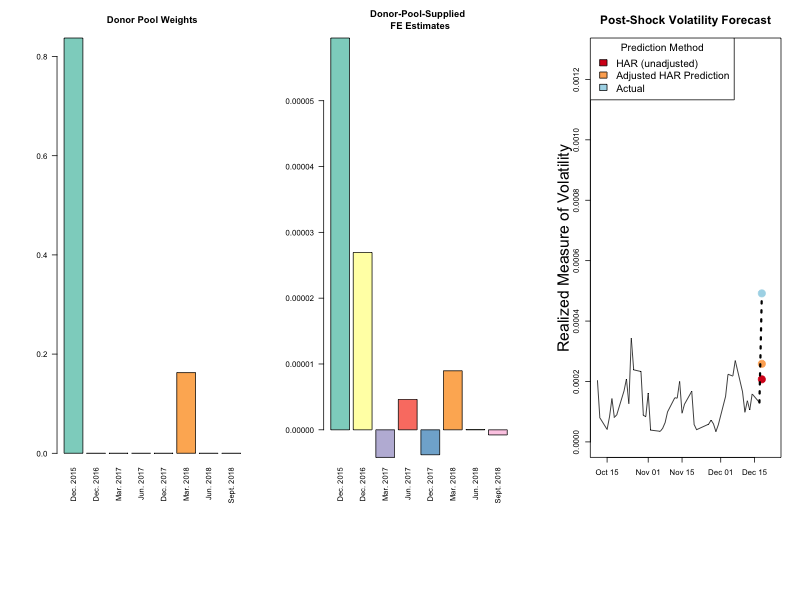
\includegraphics[scale=.3]{real_data_output_plots/savetime_SatJun151644072024__^VIX-^IRX-^XAU_^VIX_2018-12-18-2015-12-15-2016-12-13-2017-03-14-2017-06-13-2017-12-12-2018-03-20-2018-06-12-2018-09-25.png}}{demonstration.mp4}
        \caption{Click the image above to see a video of the R package's functionality.}
    \end{figure} 




\end{frame}

\begin{frame}\frametitle{LLMs}
    Use NLP to identify donors.

    \begin{figure}[H]
        \begin{center}
          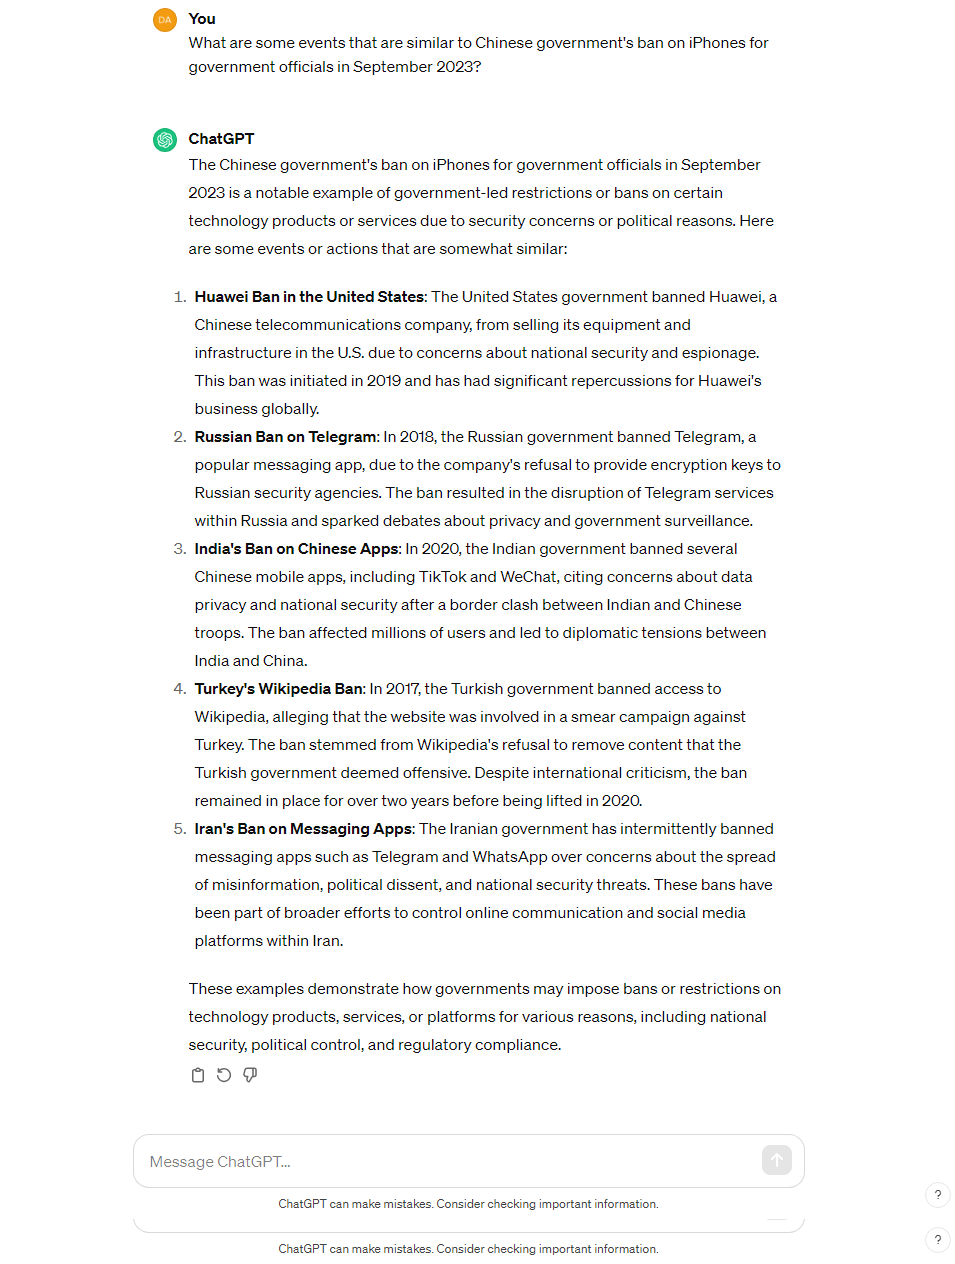
\includegraphics[scale=.18]{iphone.png}
          \end{center}
        \end{figure}


     
\end{frame}

\section{How can we trust this?}

\begin{frame}\frametitle{Robustness of the Approach}
    What assurances do we have that the method will be good?

    \bigskip

    Some ideas here:

    \begin{enumerate}
    \item multiverse
    \item permute donors
    \end{enumerate}

    \end{frame}


\section{Future directions for Forecasting Amid Shocks}



\begin{frame}
We shall group the extensions into five buckets:
\begin{itemize}
    \item How much can we automate?
    \item Alternatives for fixed effect estimation
    \item Alternative estimators and estimands
    \item What can you do with a volatility forecast?
    \item Where else is distanced-based weighting useful?
    \item Can we extend the results of \parencite[][]{bodilsen2023exploiting}
\end{itemize}
\end{frame}


\begin{frame}{How much can we automate?}

    What if the covariates are difficult to specify?

    \bigbreak
    Proposed solution:

    \bigbreak

    Use shrinkage estimation to detect fleeting signals in the cross section of $a_{t}^{2}$ \parencite[][]{chinco2019sparse}. 
\end{frame}

% \begin{frame}
% \frametitle{Alternative Ways of Estimating Fixed Effects}
% High-frequency data?

% \begin{itemize}

% \item{Realized GARCH with High-Frequency Data}

% \item{Stochastic Volatility}
% \end{itemize}
% \end{frame}

% \begin{frame}
%     \frametitle{Alternative Estimators and Estimands in Volatility Modeling}
%     \begin{itemize}
        
%         \item Factors used as covariates
%         \item Overnight returns instead of open-to-close
        
%         \item Signal Recovery Perspective \parencite{ferwana2022optimal}
        
%         \item Stochastic Volatility: Correlation between errors
%         \item Multivariate GARCH
        
%         \end{itemize}
% \end{frame}

% \begin{frame}
%     \frametitle{What can you do with a volatility forecast?}
%     \begin{itemize}
%         \item{Value-at-Risk using SVF-based $\hat\sigma^{2}_{t}$}
%         \end{itemize}
% \end{frame}

\section{Directions and Limitations}

\begin{frame}
    \frametitle{Limitations of what we're currently doing}
    \begin{itemize}
        \item Our real data examples cannot be scaled up due to the need to for human involvement in donor and covariate curation
        \item We assume that the exogenous variables (distinct from the covariates) are known at time $T_{i}^{*}$
        \item Heterogeneity of DGPs
        \item Forecast evaluation
        \item We could only truly explore a subset of the vast parameter space.
        \item The failure of distance-based weighting to extrapolate
    \end{itemize}
\end{frame}

\begin{frame}
    \frametitle{New Frontiers in Distance-based Weighting}
    \begin{itemize}
        \item Forecast conditional upon the shock \textit{prior} to the shock's arrival
        \item Integrate lessons from literature on under/over reactions to information shocks \parencite[][]{jiang2017information}
        \item{Distance-based Weighting of Impulse Response Functions}
        \end{itemize}
\end{frame}



\begin{frame}{Distance-based Weighting of Impulse Response Functions}
    Suppose 
    \begin{itemize}
        \item We have a collection of $p$-variate time series of lengths $T_{i}, i=1,2,...n+1$.
        \item We are interested in the response of variable $r$ to shocks in variable $j$, $1\leq r \leq j \leq p$. 

    \end{itemize}
    
\bigbreak
There many ways to estimate $IRF_{1}(r,j).$

\bigbreak
Can we somehow aggregate the estimates $\widehat{IRF}_{i}(r,j)$, $i = 2,3,...,n+1$? \\

Additional research questions:
\begin{itemize}
    \item What DGP would best motivate/justify such a method?
    \item Which method of IRF estimation would perform best?

\end{itemize}
\end{frame}


%We analyze the real data example with Brexit included.

% \begin{figure}[H]
%     \begin{center}
%       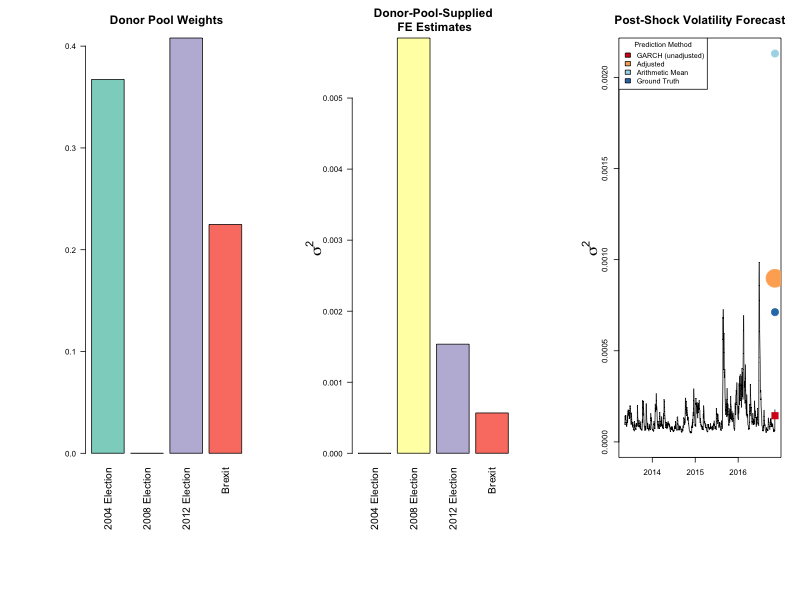
\includegraphics[scale=.32]{real_data_output_plots/savetime_SunMar172251232024_IYG_6B=F-CL=F-^VIX-^IRX-^FVX-^TNX-^TYX_^VIX_2016-11-08-2004-11-02-2008-11-04-2012-11-06-2016-06-22.png}
%       \end{center}
%     \end{figure}
    

\begin{frame}[t,allowframebreaks]
    \frametitle{References}
    % https://latex.org/forum/viewtopic.php?t=13344
    % \bibliographystyle{plainnat}
    % \bibliography{synthVolForecast}

\printbibliography[heading=none]
\end{frame}

\end{document}